\chapter{AI Component Design}
\label{chap:ai-component-design}

% \section{Software Development Methodology}
% \label{section:software-development-methodology}
% <TIP: Describe your software development methodology in this section. />

% \section{Technology Stack}
% \label{section:technology-stack}
% <TIP: Describe your technology stack here. See the following example from ThaiProgrammer.org />
% \begin{figure}[h]
%     \centering
%     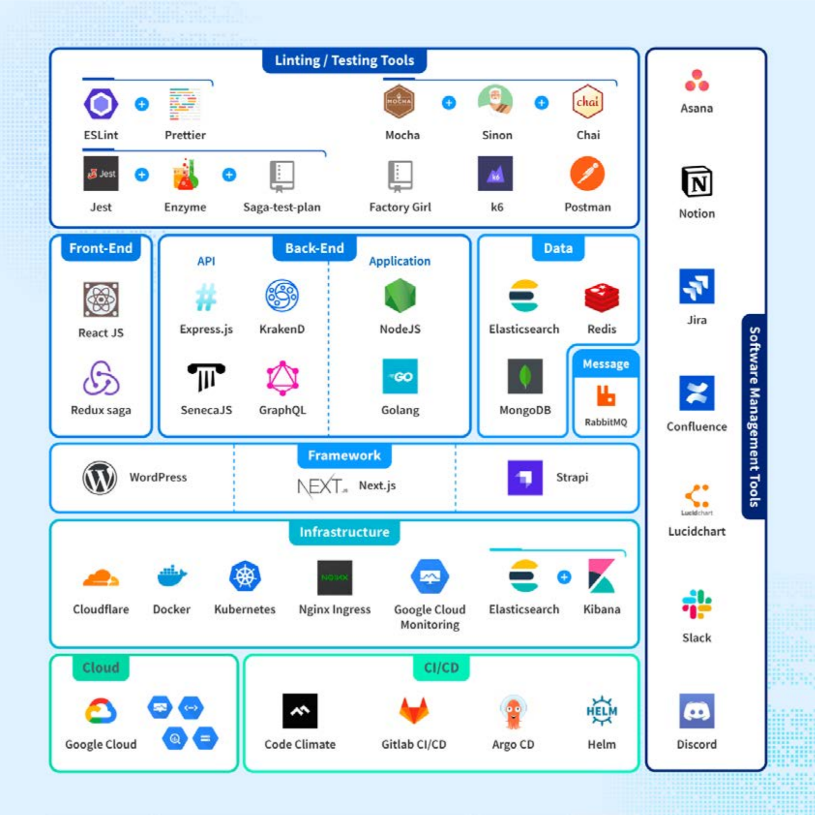
\includegraphics[width=0.5\textwidth]{examples/tech-stack.png}
%     \caption{Example technology stack}
% \end{figure}

% \section{Coding Standards}
% \label{section:coding-standards}
% <TIP: Describe your coding standard for this project here. />

% \section{Progress Tracking Report}
% \label{section:progress-tracking-report}
% <TIP: Show that you have been working on this project overtime.
% It can be in the form of a burndown chart or a contribution graph from GitHub./>

\section{Business Context \& AI Integration}

\label{section:business-context-ai-integration}
\begin{figure}[H]
    \centering
    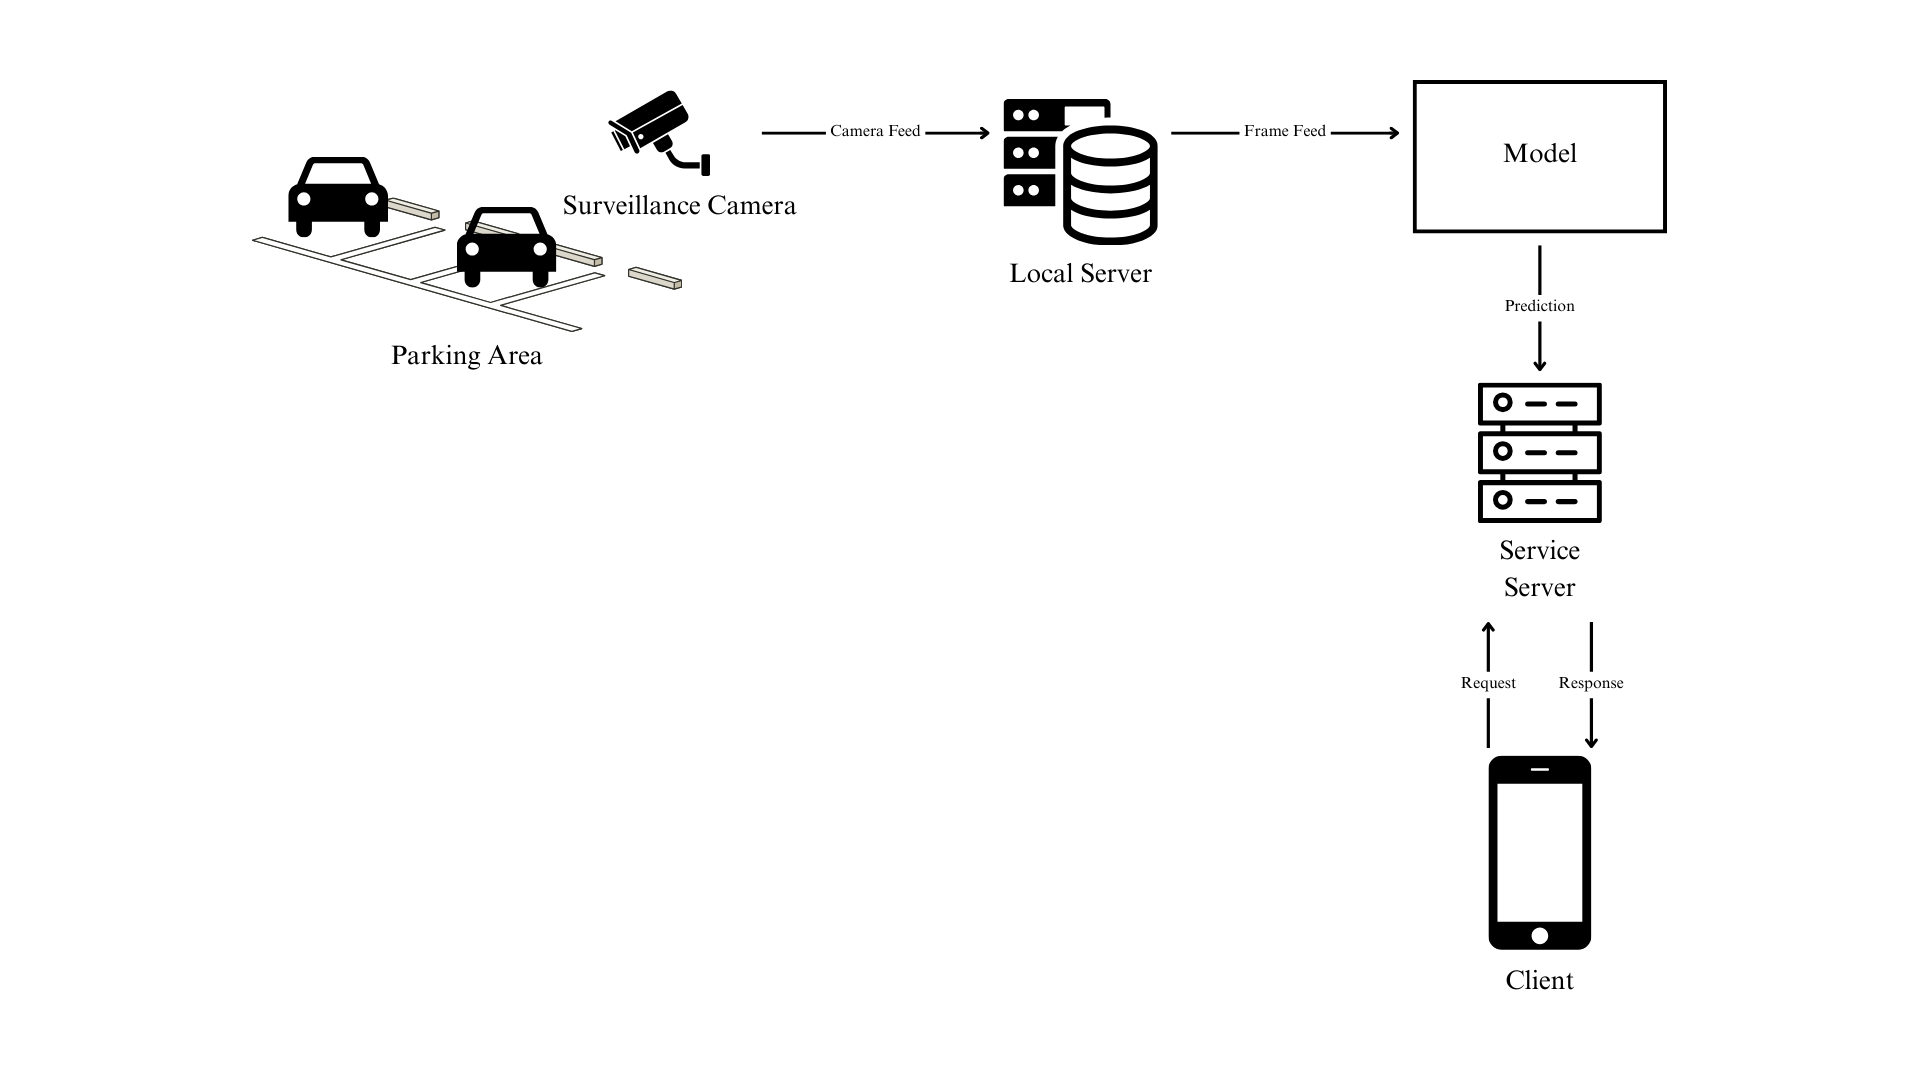
\includegraphics[width=\textwidth,keepaspectratio]{diagrams/system-flow/overview-system-flow.png}
    \caption{Overview System Flow}
    \label{fig:overview-system-flow}
\end{figure}

\begin{figure}[H]
    \centering
    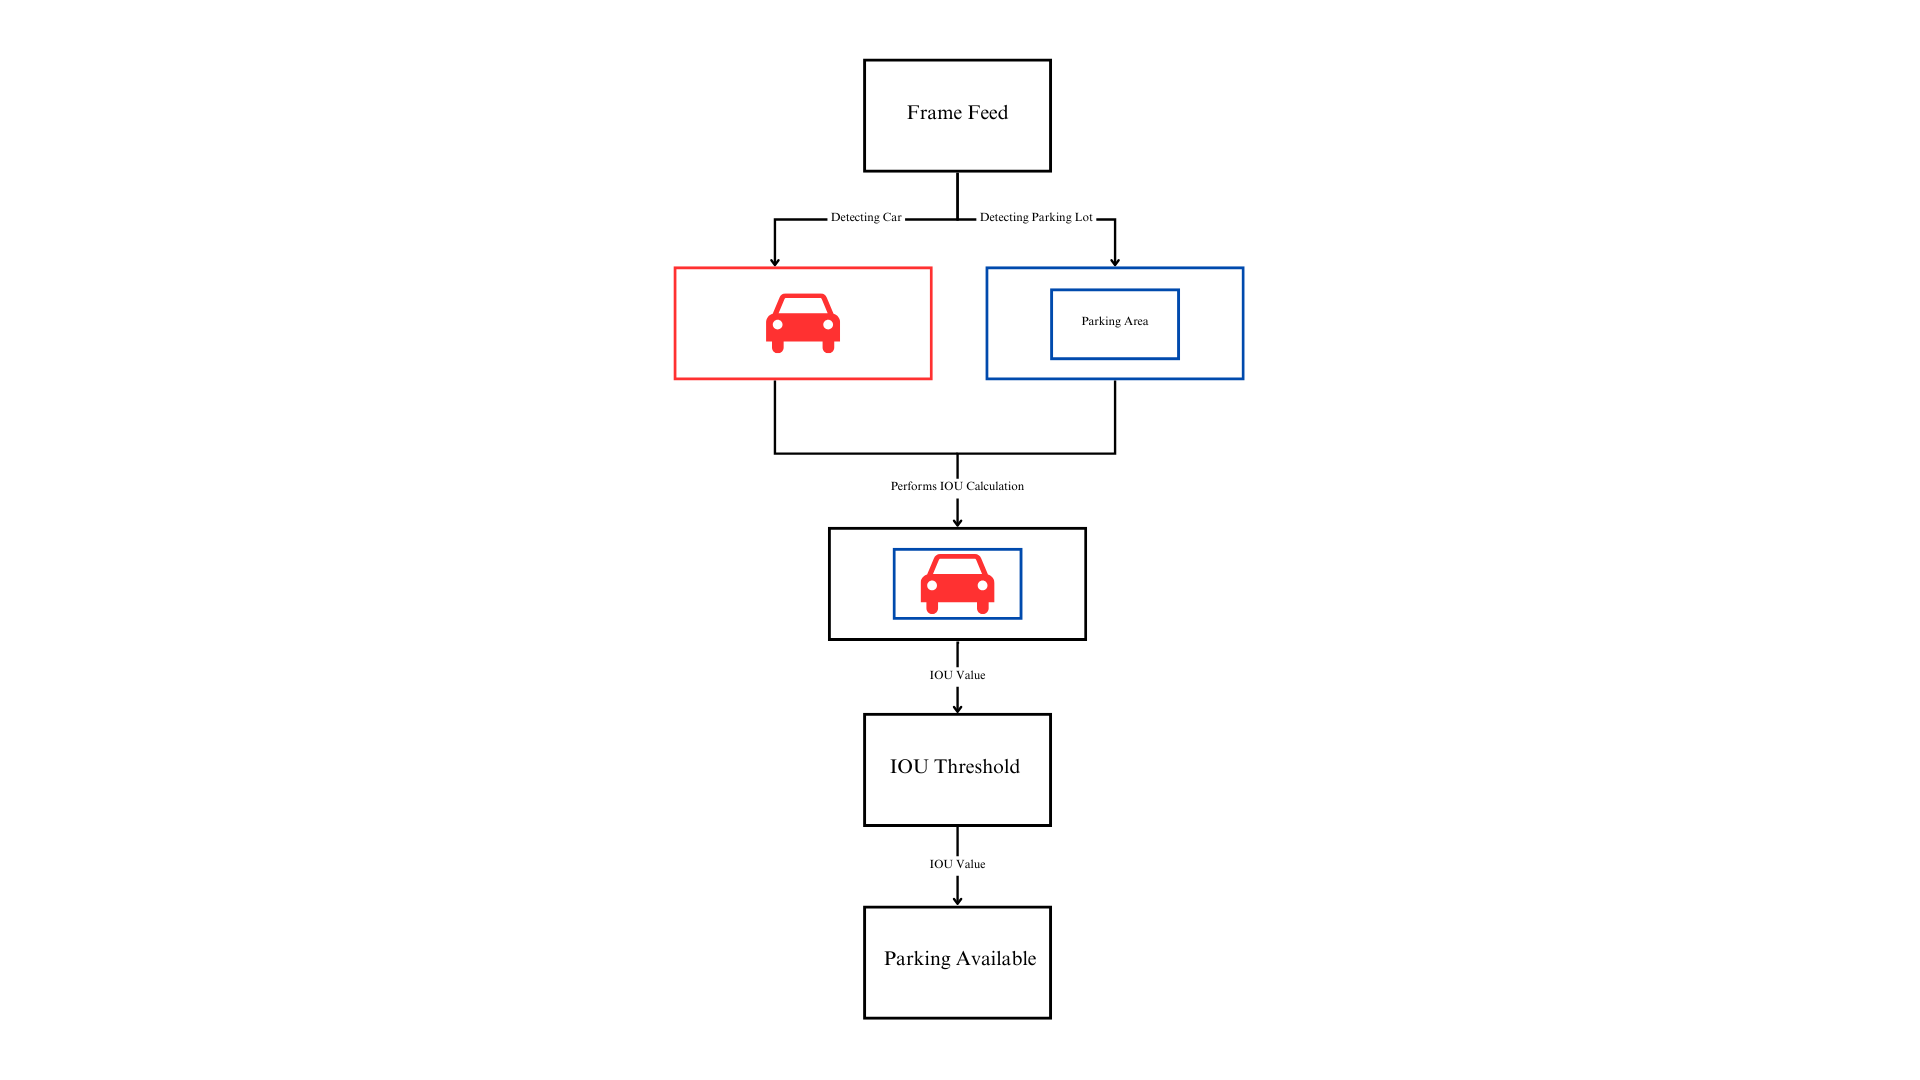
\includegraphics[width=\textwidth,keepaspectratio]{diagrams/system-flow/model-flow.png}
    \caption{Detection Model Flow}
    \label{fig:model-flow}
\end{figure}


KU Parking has integrated AI for the detection of available parking spots. Figure \ref{fig:overview-system-flow} provides a system overview: surveillance cameras monitor the parking area, feeding video to a local surveillance footage server. Periodically, individual frames from the video stream are extracted and processed by the model (as outlined in Figure \ref{fig:model-flow}). The model performs object detection to locate both cars and parking spaces within the image. Subsequently, it calculates the Intersection over Union (IoU), a metric quantifying the overlap between each detected vehicle's bounding box and the defined area of a parking spot. By comparing the IoU against a set threshold, the system determines if a vehicle significantly occupies a parking space, thus indicating its availability. This output is served to the client by the service server.

By integrating a detection model, KU Parking can reduce the cost of installing a parking indication system by leveraging existing infrastructure. To inform users, parking availability requires continuous monitoring, as the availability and usage of parking spots can change throughout the day. The model helps automate this continuous monitoring process by analyzing feeds, providing up-to-date information on parking spot occupancy. The incorrect detections typically result in minor user frustration rather than significant damage.

\section{Goal Hierarchy}
\label{section:goal-hierarchy}

The tables in this section outline the goals for the KU Parking system at different levels: Organizational (Table \ref{tab:organization-goal}), System (Table \ref{tab:system-goal}), User (Table \ref{tab:user-goal}), and AI Model (Table \ref{tab:ai-model-goal}). Each table details the goal, how it will be measured, the data collection methods, and how the goal will be operationalized.

\begin{table}[H]\caption{Organizational Goals of KU Parking}
    \label{tab:organization-goal}
    \centering
    \resizebox{\textwidth}{!}{ 
        \begin{tabular}{|p{4cm}|p{4cm}|p{4cm}|p{4cm}|} 
            \hline
            \textbf{Organizational Goals} & \textbf{Identified Measure} & \textbf{Data Collection} & \textbf{Operationalization} \\
            \hline
            Enhance on-campus driver experience & User satisfaction rating & User feedback survey, app usage analytics & Regular user satisfaction surveys and Usage frequency \\
            \hline
            Promote smart campus development with cost-effective tech & System installation and maintenance cost and alternatives & Record of KU Parking development and deployment expenses & Compare installation and operational costs to alternatives \\
            \hline
        \end{tabular}
    }
\end{table}

\begin{table}[H]\caption{System Goals of KU Parking}
    \label{tab:system-goal}
    \centering
    \resizebox{\textwidth}{!}{ 
        \begin{tabular}{|p{4cm}|p{4cm}|p{4cm}|p{4cm}|} 
            \hline
            \textbf{System Goals} & \textbf{Identified Measure} & \textbf{Data Collection} & \textbf{Operationalization} \\
            \hline
            Provide availability of the parking spots & Detection accuracy, latency & Model output compare to real status & Percentage of correct indication \\
            \hline
            Presenting alternative parking area & Number of parking between parking area & Logs of number of parking car in each parking area & Compare parking data between parking areas \\
            \hline
        \end{tabular}
    }
\end{table}

\begin{table}[H]\caption{User Goals of KU Parking}
    \label{tab:user-goal}
    \centering
    \resizebox{\textwidth}{!}{ 
        \begin{tabular}{|p{4cm}|p{4cm}|p{4cm}|p{4cm}|} 
            \hline
            \textbf{User Goals} & \textbf{Identified Measure} & \textbf{Data Collection} & \textbf{Operationalization} \\
            \hline
            Quickly find optimal available parking spaces & User satisfaction rating & User feedback survey, app usage analytics & Regular user satisfaction surveys and Usage frequency \\
            \hline
        \end{tabular}
    }
\end{table}

\begin{table}[H]\caption{AI Model of KU Parking}
    \label{tab:ai-model-goal}
    \centering
    \resizebox{\textwidth}{!}{ 
        \begin{tabular}{|p{4cm}|p{4cm}|p{4cm}|p{4cm}|} 
            \hline
            \textbf{AI Model Goals} & \textbf{Identified Measure} & \textbf{Data Collection} & \textbf{Operationalization} \\
            \hline
            Accurately detect vacant space & Precision, recall, F1 score & Annotated images, prediction logs & Model evaluation using labeled datasets \\
            \hline
            Operate efficiently in close to real time & latency & System logs & Measure average time per image/frame \\
            \hline
        \end{tabular}
    }
\end{table}

\section{Task Requirements Analysis Using AI Canvas}
\label{section:task-requirement-analysis-using-ai-canvas}
<TIP: Describe your coding standard for this project here. />


\section{User Experience Design with AI}
\label{section:user-experience-with-ai}
<TIP: Describe your coding standard for this project here. />
